\documentclass[../../../../../../Assignments.tex]{subfiles}

% \documentclass{book}
% \usepackage{pgfplots}
% \pgfplotsset{compat=1.17}


\begin{document}
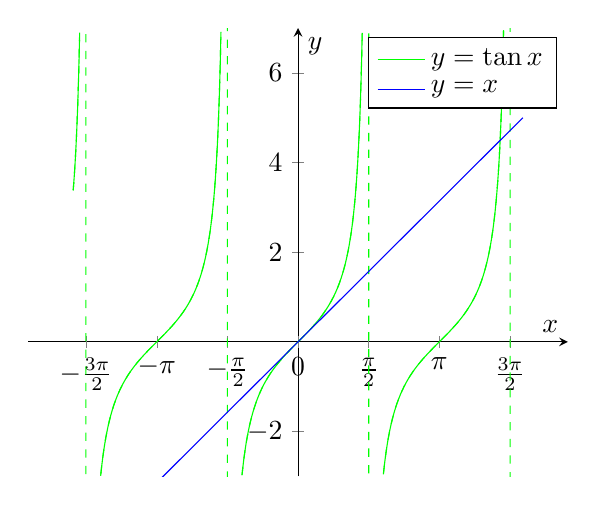
\begin{tikzpicture}
    \begin{axis}[
        axis lines=center,
        samples=1000,
        xlabel={\(x\)},
        xmin=-6,xmax=6,
        xtick=\empty,
        extra x ticks      ={-1.5 * pi          , -pi     , -0.5 * pi         , 0, 0.5 * pi         , pi     , 1.5 * pi},
        extra x tick labels={\(-\frac{3\pi}{2}\), \(-\pi\), \(-\frac{\pi}{2}\), 0, \(\frac{\pi}{2}\), \(\pi\), \(\frac{3 \pi}{2}\)},
        ylabel={\(y\)},
        ymin=-3,ymax=7,
        legend cell align={left},
    ]
        % Asymptote lines are part of the graph, so first draw a dashed graph
        \addplot [green, dashed, forget plot] {tan(deg(x))};    % forget plot: no legend
        % then draw a normal one on top, but restrict y so no asymptote is drawn
        \addplot [green, restrict y to domain=-3:7] {tan(deg(x))};
        \addlegendentry{\(y = \tan{x}\)}

        \addplot[blue, samples=10] {x};
        \addlegendentry{\(y = x\)}
    \end{axis}
\end{tikzpicture}
\end{document}
